\documentclass[a4paper,12pt,oneside,final]{report}
%\usepackage{geometry}                % See geometry.pdf to learn the layout options. There are lots.
%\geometry{landscape}                % Activate for for rotated page geometry
%\usepackage[parfill]{parskip}    % Activate to begin paragraphs with an empty line rather than an indent
\usepackage{graphicx}
% \usepackage{amssymb}
\usepackage{epstopdf}
\usepackage[utf8]{inputenc}
\usepackage{titlesec}
\usepackage[titletoc]{appendix}
\titleformat{\chapter}[hang]{\bf\Huge}{\thechapter}{1cm}{}

\pagestyle{plain}
% -------------------- this stuff for code --------------------

\usepackage{anysize}
\marginsize{30mm}{30mm}{20mm}{20mm}

\newenvironment{formal}{%
  \def\FrameCommand{%
    \hspace{1pt}%
    {\color{blue}\vrule width 2pt}%
    {\color{formalshade}\vrule width 4pt}%
    \colorbox{formalshade}%
  }%
  \MakeFramed{\advance\hsize-\width\FrameRestore}%
  \noindent\hspace{-4.55pt}% disable indenting first paragraph
  \begin{adjustwidth}{}{7pt}%
  \vspace{2pt}\vspace{2pt}%
}
{%
  \vspace{2pt}\end{adjustwidth}\endMakeFramed%
}

\newenvironment{changemargin}[2]{\begin{list}{}{%
\setlength{\topsep}{0pt}%
\setlength{\leftmargin}{0pt}%
\setlength{\rightmargin}{0pt}%
\setlength{\listparindent}{\parindent}%
\setlength{\itemindent}{\parindent}%
\setlength{\parsep}{0pt plus 1pt}%
\addtolength{\leftmargin}{#1}%
\addtolength{\rightmargin}{#2}%
}\item }{\end{list}}

\usepackage{color}
\usepackage{dsfont}
\usepackage[bitstream-charter]{mathdesign}
\usepackage[scaled]{helvet}
\usepackage{inconsolata}


\definecolor{colKeys}{rgb}{0,0,0.9} 
\definecolor{colIdentifier}{rgb}{0,0,0} 
\definecolor{colString}{rgb}{0.7,0,0} 
\definecolor{colComments}{rgb}{0,0.6,0} 
\usepackage{listings}
\lstset{
  language=python,
  stringstyle=\color{colString},
  keywordstyle=\color{colKeys},
  identifierstyle=\color{colIdentifier},
  commentstyle=\color{colComments},
  numbers=left,
  tabsize=4,
  frame=single,
  breaklines=true,
  basicstyle=\small\ttfamily,
  numberstyle=\tiny\ttfamily,
  framexleftmargin=0mm,
  xleftmargin=7mm,
  xrightmargin=7mm,
  frameround={tttt},
  captionpos=b
}

%% Headers and footers
\usepackage{fancyhdr}
\usepackage[section]{placeins}
\pagestyle{fancy}
\fancyhf{}
\addtolength{\headwidth}{30pt}
\addtolength{\headwidth}{30pt}
\renewcommand{\headrulewidth}{0.4pt} % thickness of the header line
\renewcommand{\footrulewidth}{0.4pt} % thickness of the footer line
\renewcommand{\chaptermark}[1]{\markboth{#1}{#1}} % chapter name
\renewcommand{\sectionmark}[1]{\markright{\thesection\ #1}}  % section name
\lhead[\fancyplain{}{\bf\thepage}]{\fancyplain{}{\bf\rightmark}} % display header
\rhead[\fancyplain{}{\bf\leftmark}]{\fancyplain{}{}} % display header
\fancyfoot[C]{\bf\thepage} % display footer (page number)
\fancyfoot[R]{\bf\today} % display footer (date)
\fancypagestyle{plain}{ 
	\fancyhead{} \renewcommand{\headrulewidth}{0pt}
}
\newcommand{\clearemptydoublepage}{\newpage{\pagestyle{plain}\cleardoublepage}}

\usepackage[T1]{fontenc}
\usepackage{enumerate}
\usepackage{afterpage,lastpage,fancyhdr}
\usepackage[includeheadfoot,margin=2.5cm]{geometry}
\geometry{letterpaper}                   % ... or a4paper or a5paper or ... 

% -------------------- end of code stuff --------------------



\DeclareGraphicsRule{.tif}{png}{.png}{`convert #1 `dirname #1`/`basename #1 .tif`.png}

\makeatletter \def\thickhrulefill{\leavevmode \leaders \hrule height 1pt\hfill
\kern \z@} \renewcommand{\maketitle}{
    \begin{titlepage}
    \let\footnotesize\small \let\footnoterule\relax \parindent \z@ \reset@font
    \null\vfil
    \vspace{-20mm}
    \begin{center}
    {\small \scshape Imperial College London}
    \end{center}
    \vspace{0.5cm}
	\begin{minipage}{\textwidth}
		\vspace{1cm}
		%\noindent\rule[0ex]{\textwidth}{4pt} \\
		%\flushright
		\center
		\@title
		\\ \vspace{4mm}
		%\noindent\rule[0ex]{\textwidth}{4pt} \\
	\end{minipage}
	\vspace{2cm}
	\begin{center}
		
\includegraphics[width=70mm,]{logo_imperial_college_london.png}
	\end{center}
	\vspace{5.4cm}
	\vspace{\stretch{1}}
	\begin{minipage}{\textwidth}
		\flushright
		{\bfseries}
		\vspace{7mm}
		\center
		\@author\\
	\end{minipage}
	\vspace{20mm}
		\flushleft
		{\bfseries}
		{\small \scshape \@date }
		\vspace{0.1cm}
		\rule{\linewidth}{.5pt}
  \end{titlepage}
  \setcounter{footnote}{1}
  \setcounter{page}{2}
}


\author{Paul Gribelyuk (pg1312, a5)}
\makeatother
\title{\Huge \#DOC417 - Advanced Computer Graphics Coursework 2}
\date{\today}

\begin{document}
\maketitle
% \tableofcontents
\listoffigures
\chapter{Generating Plots of Fresnel Reflectance}
\paragraph{}
I produced the graphs of Fresnel reflectance using iPython with the following scripts:
\begin{lstlisting}[ ]
def snell_thetaT(thetaI, etaI, etaT):
    return asin(sin(thetaI)*etaI/etaT)

def Rs(thetaI, etaI, etaT):
    thetaT = snell_thetaT(thetaI, etaI, etaT)
    numer = etaI * cos(thetaI) - etaT * cos(thetaT)
    denom = etaI * cos(thetaI) + etaT * cos(thetaT)
    return abs(numer / denom)**2

def Rp(thetaI, etaI, etaT):
    thetaT = snell_thetaT(thetaI, etaI, etaT)
    numer = etaI * cos(thetaT) - etaT * cos(thetaI)
    denom = etaI * cos(thetaT) + etaT * cos(thetaI)
    return abs(numer / denom)**2
\end{lstlisting}
The graph associated the cofficients of parallel and perpendicular reflection, $R_p$ and $R_s$ respectively, for light entering a dielectric material (with $\eta = 1.5$) is displayed in Figure \ref{fig:fresnel1}.
\begin{figure}[!h]
  \begin{changemargin}{-50mm}{-50mm}
    \center
    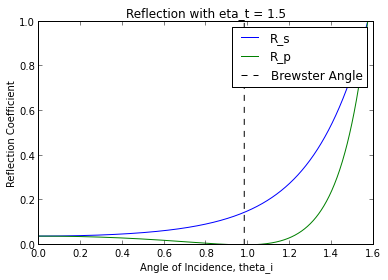
\includegraphics[scale=0.8]{fresnel1.png}
    \caption{Light entering a dielectric medium \label{fig:fresnel1}}
  \end{changemargin}
\end{figure}

The graph associated with $R_p$ and $R_s$ for light leaving a dielectric with $\eta = 1.5$ is displayed in Figure \ref{fig:fresnel2}.
\begin{figure}[!h]
  \begin{changemargin}{-50mm}{-50mm}
    \center
    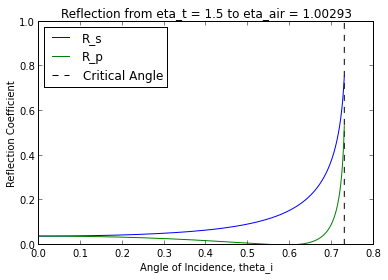
\includegraphics[scale=0.8]{fresnel2.png}
    \caption{Light leaving a dielectric medium \label{fig:fresnel2}}
  \end{changemargin}
\end{figure}
The Brewster angle, was computed to be the point where $R_p = 0$, was calculated from the plotted data to be $0.981158$ radians (56.22 degrees).  The exact value calculated from the formula $\theta_B = \arctan\left(\frac{\eta_t}{\eta_i}\right)$ is $0.981443$ radians (56.23 degrees).  The critical angle was calculated directly from the formula, $\theta_C = \arcsin\left(\frac{\eta_t}{\eta_i}\right)$, to be $0.729728$ (41.81 degrees).

\chapter{Sampling an Environment Map}
In this section I sample the Grace Cathedral environment map (EM) using the cumulative density function (CDF) as well as the analytical Phong model.
\section{Monte Carlo Sampling using CDF Inversion}
This method assumes that the luminance of the pixels forms a 2D probability density from which we can sample.  The approach is as follows:
\begin{itemize}
  \item[1] Compute average luminance in each row of the image forming a 1D probability density, \verb+rowAverages+
  \item[2] Perform CDF inversion on 1D array
  \begin{itemize}
    \item[a] Calculate $CDF(i) = ( \sum_{j=0}^{i-1} array[j] ) / (\sum_{j=0}^{len(array)} array[j])$ and $CDF(0) = 0$
    \item[b] Draw random variate $\xi$
    \item[c] Find index $k$ such that $CDF[k] \geq \xi$ and $CDF[k-1] < \xi$ via binomial search, since $CDF$ is sorted
    \item[d] $k$ is the sample according to the 1D PDF represented by the input array
  \end{itemize}
  \item[3] Perform the same 1D sampling on the selected row represented by $k$, to get another index $l$
  \item[4] The pair $(k, l)$ represent the index values of a CDF-based sample of the 2D image
\end{itemize}

I applied this technique on the Grace Cathedral environment map, with images, displayed in Figures \ref{fig:grace_cdf_64}, \ref{fig:grace_cdf_256}, \ref{fig:grace_cdf_1024}

\begin{figure}[!h]
  \begin{changemargin}{-50mm}{-50mm}
    \center
    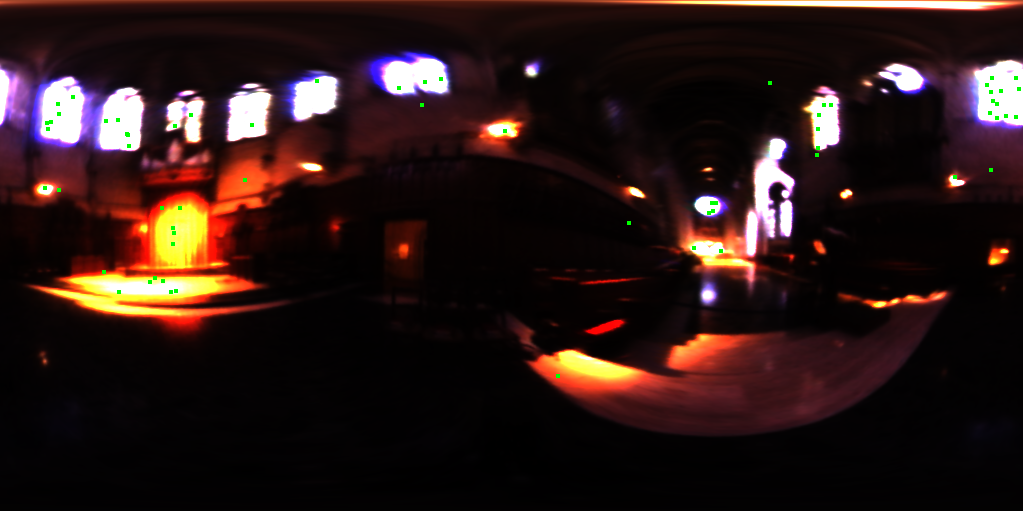
\includegraphics[scale=0.4]{grace_cdf_64.png}
    \caption{Grace Cathedral sampled via CDF Inversion with 64 samples \label{fig:grace_cdf_64}}
  \end{changemargin}
\end{figure}

\begin{figure}[!h]
  \begin{changemargin}{-50mm}{-50mm}
    \center
    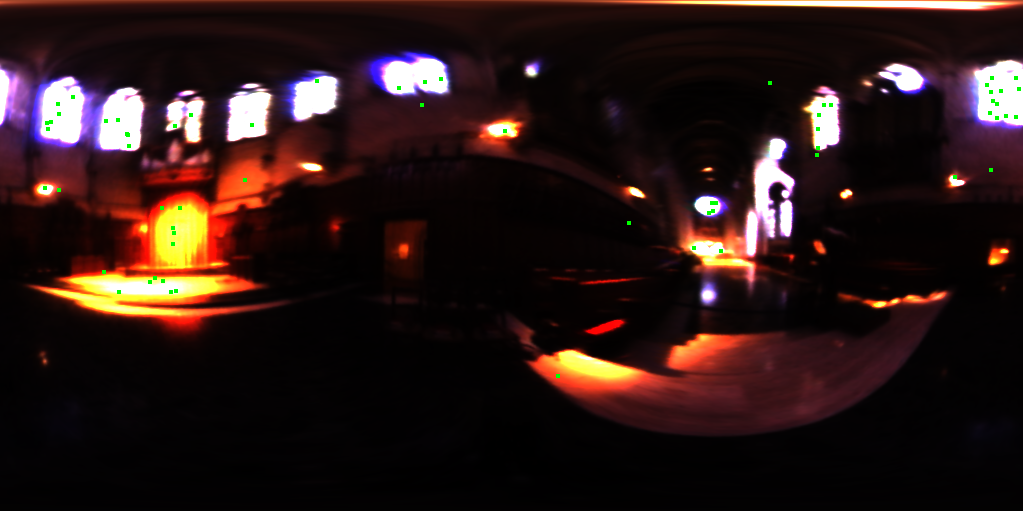
\includegraphics[scale=0.4]{grace_cdf_64.png}
    \caption{Grace Cathedral sampled via CDF Inversion with 256 samples \label{fig:grace_cdf_256}}
  \end{changemargin}
\end{figure}

\begin{figure}[!h]
  \begin{changemargin}{-50mm}{-50mm}
    \center
    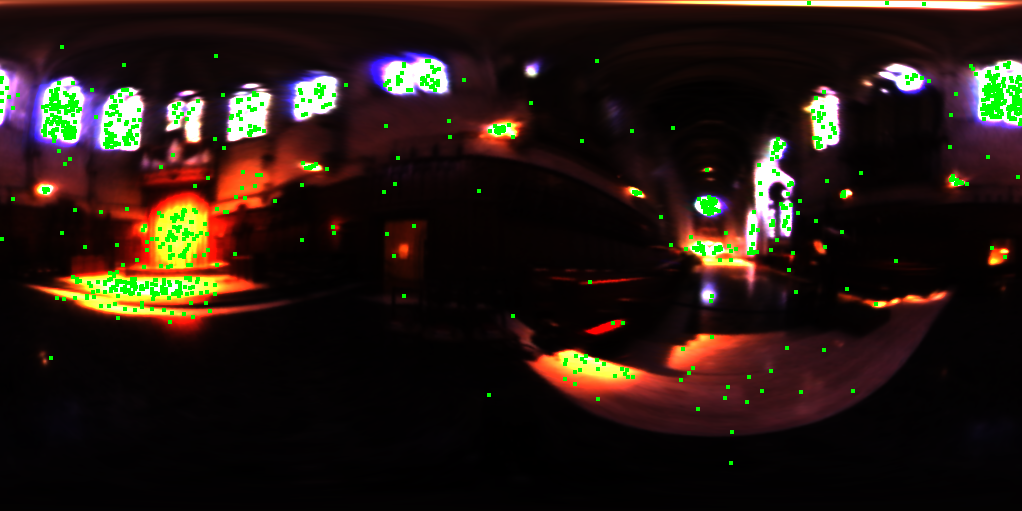
\includegraphics[scale=0.4]{grace_cdf_1024.png}
    \caption{Grace Cathedral sampled via CDF Inversion with 1024 samples \label{fig:grace_cdf_1024}}
  \end{changemargin}
\end{figure}

\section{Phong Lobe Sampling}
The Phong sampling technique is an analytical procedure, not relying on the input image data.  The formulation is as follows (exponent $n$ is an input):
\begin{itemize}
  \item[1] Draw uniform random variates $\xi_1$ and $\xi_2$
  \item[2] The corresponding sampled angular values are $(\theta, \phi) = \left(\cos^{-1}\left\{(1 - \xi_1)^{\frac{1}{n+1}}\right\}, 2\pi\xi_2\right)$
  \item[3] The corresponding indices in the latlong map are $(k, l) = \left(\frac{2\theta}{\pi} \cdot H, \frac{\phi}{2\pi} \cdot W\right)$
\end{itemize}
The images resulting from the application of this tecnique are in Figures \ref{fig:phong_256_10} and \ref{fig:phong_1024_50}.
\begin{figure}[!h]
  \begin{changemargin}{-50mm}{-50mm}
    \center
    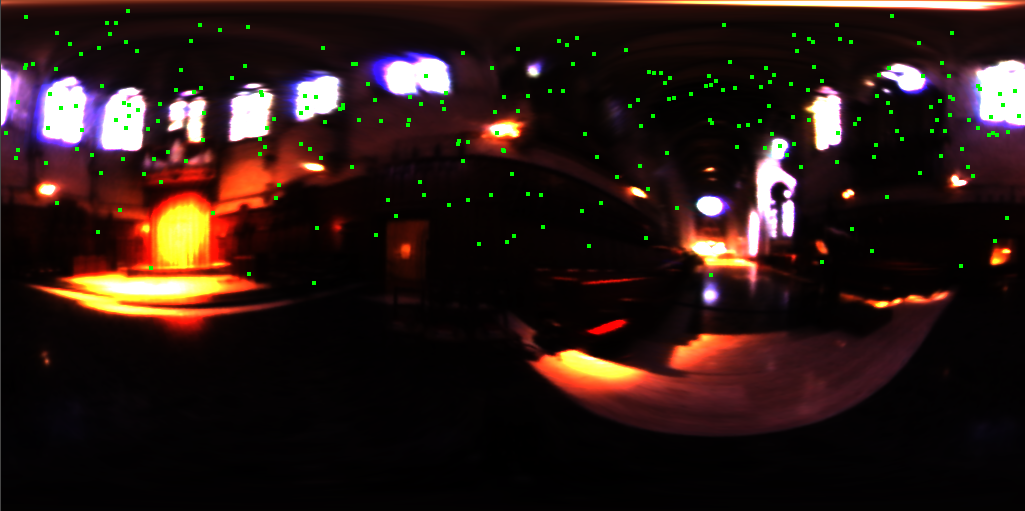
\includegraphics[scale=0.4]{grace_phong_256_10.png}
    \caption{Grace Cathedral sampled via Phong with 256 samples and $n=5$ \label{fig:phong_256_10}}
  \end{changemargin}
\end{figure}

\begin{figure}[!h]
  \begin{changemargin}{-50mm}{-50mm}
    \center
    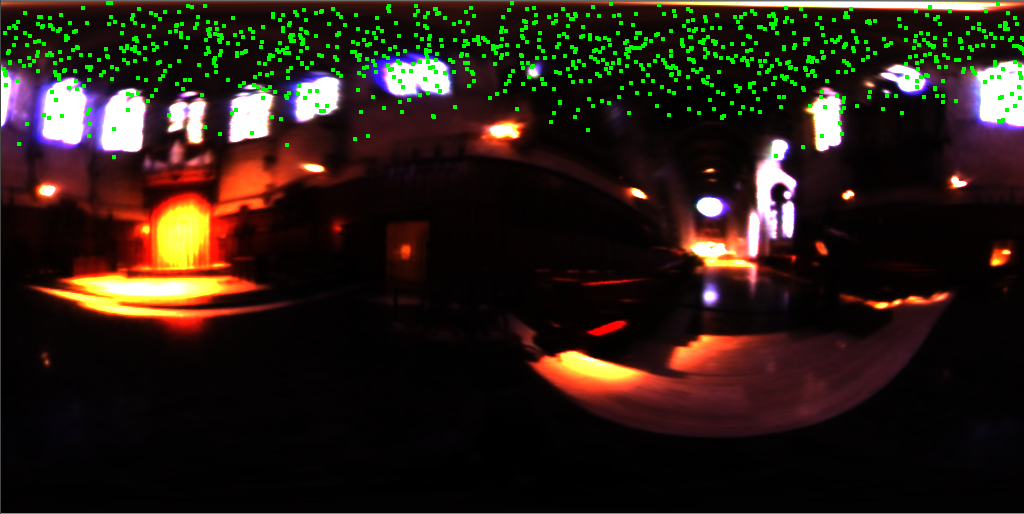
\includegraphics[scale=0.4]{grace_phong_1024_50.png}
    \caption{Grace Cathedral sampled via Phong with 1024 samples and $n=50$ \label{fig:phong_1024_50}}
  \end{changemargin}
\end{figure}

\chapter{Rendering a Sphere with EM Samples}
To render a sphere with samples drawn via CDF inversion from an environment map, we first assume that the BRDF associated with the sphere is diffuse, thus simplifying the integral equation at each point on the sphere to:
$$
L_{r, N} (\omega_r) = \frac{\int_{\Omega} L_i (\omega_i) d\omega_i}{N}\cdot \sum_{j=1}^N \frac{1}{\pi} \cos(\theta_{i,j}) NormColor_i
$$
where $d\omega_i = sin\theta d\theta d\phi$ is the solid angle, and $NormColor$ is the normalized pixel 3-vector at the sample $j$.

First, I pre-computed the intergral $\int_{\Omega} L_i (\omega_i) d\omega_i$:
\begin{lstlisting}[ ]
def precomputeIntegral(self, imageData):
    self.integral = 0.0
    luminance = np.average(imageData, axis=2)
    d_theta = math.pi / float(luminance.shape[0])
    d_phi = 2*math.pi / float(luminance.shape[1])
    for idx, v in np.ndenumerate(luminance):
      theta = d_theta * idx[0]
      d_omega = math.sin(theta) * d_theta * d_phi
      self.integral += v * d_omega
\end{lstlisting}
Next, I need to compute the sum at each point on the sphere:
\begin{lstlisting}[ ]
def monteCarloSum(self, sampleValues, spherePixel):
    self.mcSum = 0.0
    theta = spherePoint[0] * 2 * math.pi / (self.diameter + 1)
    for s in sampleValues:
      self.mcSum += cos(theta) * (s / norm(s)) / math.pi
\end{lstlisting}
Finally, I can combine these two calculations, along with a spherical to Eucliean projection, to produce pixel values.
\begin{figure}[!h]
  \begin{changemargin}{-50mm}{-50mm}
    \center
    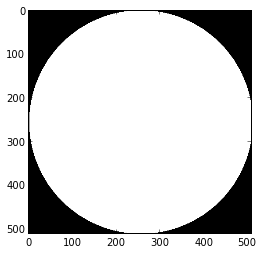
\includegraphics[scale=1]{sampled_sphere.png}
    \caption{Mapping of MC Samples onto Sphere \label{fig:sampled_sphere}}
  \end{changemargin}
\end{figure}

\end{document}  
